\section{基于Bagging的集成}
\label{sec:ensemble-bagging}

单棵树的预测可能对训练样本很敏感。例如，根节点上两个候选分裂的得分很接近，替换少量训练记录就可能让另一分裂胜出；后续节点收到的样本随之改变，最终预测也可能不同。这正是上一节说的“方差大”。若能从同一总体反复抽取多份独立的训练集，分别建树后平均，各树因样本偶然性产生的波动就会相互抵消。困难在于现实中通常只有一份训练数据，不可能真的回到总体重新采样。

统计学的\emph{自助法}（bootstrap）提供了一个巧妙的替代：既然拿不到总体，就把手头这份样本当作总体的“缩影”，从中\emph{有放回地}重复抽样。具体做法是从$n$条记录里每次随机抽一条、记下后放回，连抽$n$次，得到一份同样大小的“自助样本”。由于是有放回抽取，同一条记录可能被抽中两三次，另一些记录则一次都没被抽中，于是每份自助样本都是原数据的一个略有不同的版本，模拟了“换一批数据”的效果。\term{装袋法}（bootstrap aggregating, Bagging）就是从现有训练集抽取多份自助样本，分别训练成员，再对数值预测取平均或对类别投票。重采样让同一学习算法看到不同的记录组合，聚合则让一次样本扰动不再独自决定最终预测。若所有成员在同一区域都存在相同偏差，平均仍会保留这个偏差；Bagging主要针对的是训练扰动带来的波动，因此最适合本身容易波动（低偏差、高方差）的学习器，如深的决策树\scite{breiman1996bagging}。

\subsection{Bagging}
\label{sec:ensemble-bagging-bootstrap}

\subsubsection{模型结构}

Bagging保留$M$个由同一基学习器训练的成员，预测时按固定规则聚合。回归采用等权平均，分类采用多数投票或同类概率平均；成员之间没有逐轮修正关系，组合层也不再学习一组权重。成员的函数形式由基学习器决定，下面用自助采样使同一算法产生不同的成员。

图\ref{fig:ensemble-error-dependence}说明平均为何需要成员之间存在差异。成员各自的波动可能在平均中抵消；如果所有成员都犯同一种错误，重复增加这样的成员仍会保留共同误差。

\begin{figure*}[htbp]
  \centering
  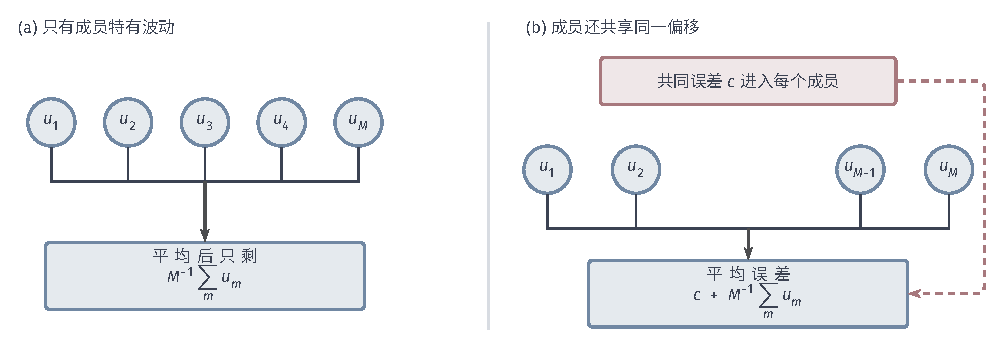
\includegraphics[width=169.000mm]{figures/04-classic-models/00-shared/tikz/ensemble-error-dependence/figure.pdf}
  \caption{成员误差依赖与平均的作用。左图表示只有成员特有波动时，平均可以随成员数增加而削弱这些波动；右图表示所有成员还共享误差$c$时，共同项仍保留在平均预测中。图中成员数量与符号只用于说明机制，不表示实测误差。}
  \label{fig:ensemble-error-dependence}
\end{figure*}

\subsubsection{参数学习}

对第$m$个成员，从$\{1,\ldots,n\}$中独立、等概率、有放回地抽取$n$次索引，所得多重集合记为$I^{(m)}$。有放回抽样使部分记录重复进入成员训练，也使部分记录留在该成员之外。学习算法$\mathcal{A}$在相应自助样本上训练出
\[
  h_m=\mathcal{A}\!\left(D_n^{(m)}\right),
  \qquad
  D_n^{(m)}=\{(\bm{x}_i,y_i):i\in I^{(m)}\}.
\]
回归通常平均$h_m(\bm{x})$；分类可以投票，也可以在成员输出具有同一语义时平均逐类得分或概率。可以改变自助样本大小或采用其他成员算法。此时仍需检验重采样是否使成员在新样本上产生互补预测。

\paragraph{构造袋外预测}

一份大小为$n$的标准自助样本没有抽中原始样本$i$的概率为
\begin{equation}
  \mathbb{P}\!\left(i\notin I^{(m)}\right)
  =
  \left(1-\frac{1}{n}\right)^n
  \longrightarrow e^{-1}.
  \label{eq:ensemble-oob-probability}
\end{equation}
因此，每个成员平均约有$36.8\%$的原始样本未参与其训练。这个副产品非常有用：评估模型通常要另外留出一份验证集，而Bagging免费送来了一份——对某个成员而言，那些它没见过的样本正好可以用来检验它，既不必额外切分数据，也没有浪费训练记录。这些样本构成该成员的\term{袋外样本}（out-of-bag sample, OOB sample）。反过来，对每个训练样本$i$，可以只收集没有使用它训练的成员预测。令
\[
  \mathcal{M}_{i}^{\mathrm{OOB}}
  =\{m:i\notin I^{(m)}\},
\]
当$\mathcal{M}_{i}^{\mathrm{OOB}}$非空时，回归的袋外预测可写为
\begin{equation}
  \widehat{y}_{i}^{\mathrm{OOB}}
  =
  \frac{1}{|\mathcal{M}_{i}^{\mathrm{OOB}}|}
  \sum_{m\in\mathcal{M}_{i}^{\mathrm{OOB}}}h_m(\bm{x}_i),
  \label{eq:ensemble-oob-prediction}
\end{equation}
分类则对同一成员集合投票或平均类别输出。图\ref{fig:ensemble-bagging-oob}按样本收集符合条件的成员：每个样本的袋外预测由其未参与训练的成员子集给出，子集随样本变化。

\begin{figure*}[htbp]
  \centering
  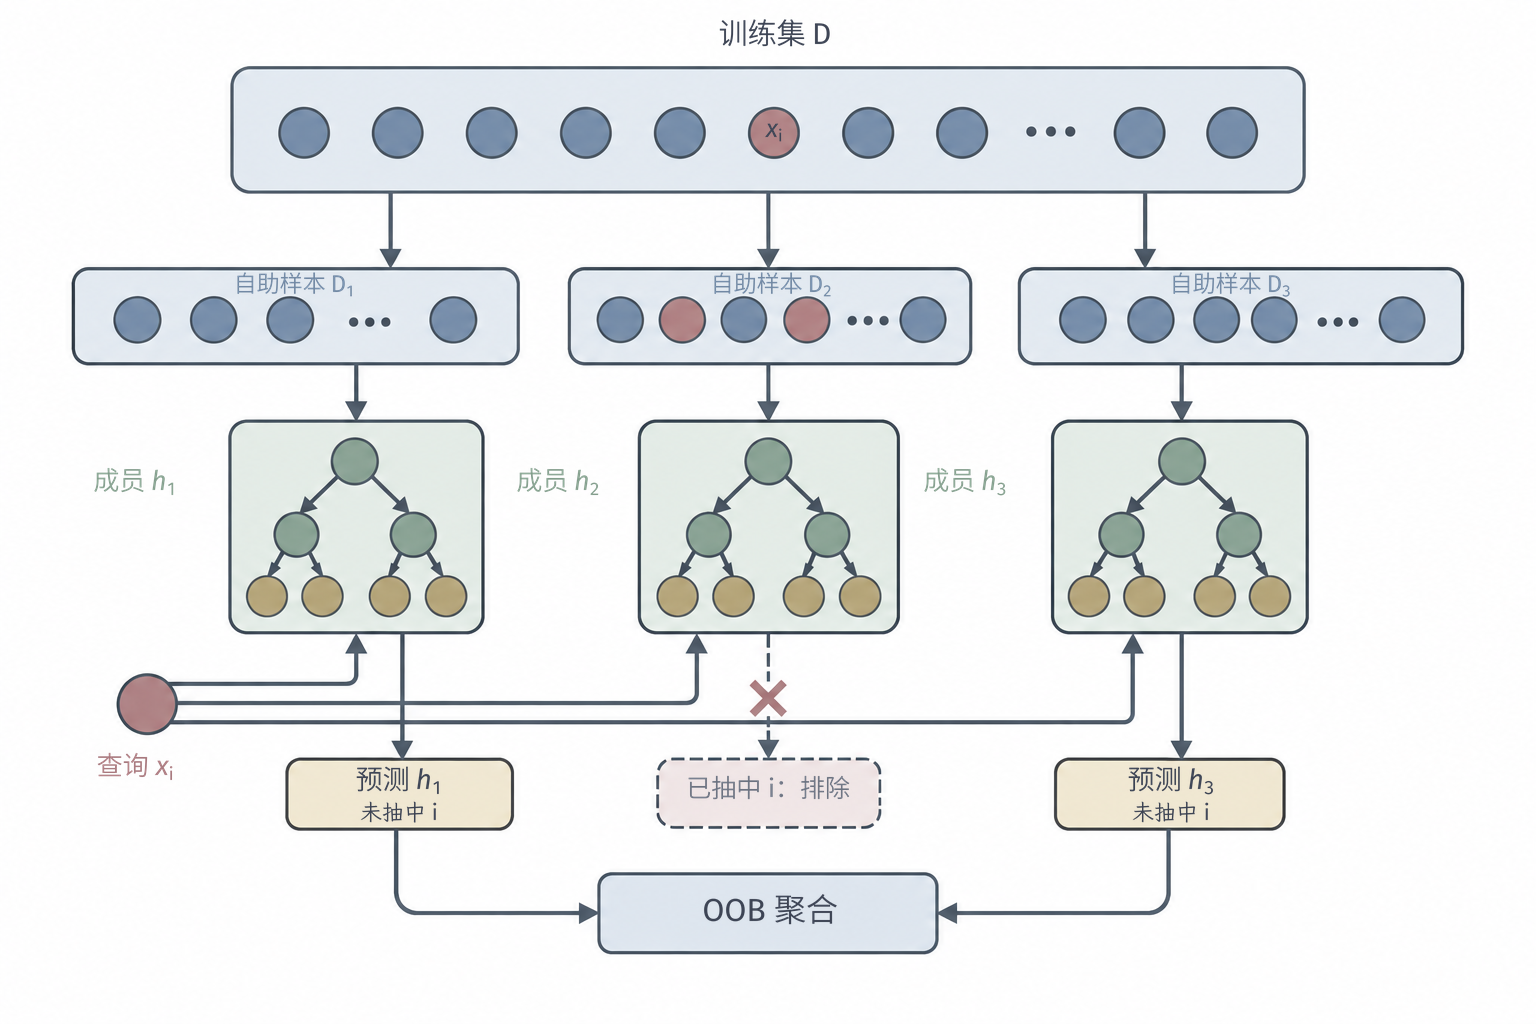
\includegraphics[width=130.048mm]{figures/04-classic-models/00-shared/generated/ensemble-bagging-oob/figure.png}
  \caption{Bagging训练与袋外预测。每个成员只使用其自助样本训练；对训练样本$\bm{x}_i$，袋外预测只聚合未抽中$i$的成员。索引与集合展示样本和成员的对应关系；成员数有限时，各样本得到的袋外预测数量不同。}
  \label{fig:ensemble-bagging-oob}
\end{figure*}

袋外预测使当前标签与产生该预测的成员训练分离，可用于绘制树数—损失曲线、内部误差估计和置换重要性。可用成员数随机变化，自助训练集又相互重叠，这一数据结构与固定折的交叉验证不同。成员数很小时，某些样本可能没有足够的袋外预测。

反复用袋外结果选择结构、树数或特征处理，会使袋外误差成为开发证据；最终冻结流程需要另用测试数据评价。时间序列、分组样本或空间相关数据还要求自助抽样尊重依赖单位；逐行重采样会破坏原有数据结构。袋外结果的解释还依赖抽样单位与未来使用的数据制度。

\paragraph{选择成员规模与训练预算}

给定原数据后，独立的重采样及训练可分配给不同计算单元。评价并行收益时，需要同时计入总工作量与实际经过时间：若单个成员的训练和预测成本分别为$C_{\mathrm{train}}$与$C_{\mathrm{pred}}$，朴素实现的总工作量仍约随$M C_{\mathrm{train}}$和$M C_{\mathrm{pred}}$增长。模型存储也通常随成员数量增加。

在固定训练集上增加独立随机成员，主要减少有限次抽样的Monte Carlo误差；等权平均逐渐逼近该随机训练机制的期望预测。原数据的抽样误差和模型失配仍影响这一期望，共同误差也会留在组合中。实践中可以观察袋外损失随成员数的变化，在曲线趋于稳定后停止增加成员，但这个停止规则也属于模型选择过程。

可以用一个固定输入处的简化误差模型看清这一区别。设第$m$个成员相对真实回归均值的误差为$b+C+U_m$，其中$b$为固定偏差，$C$为所有成员共享的零均值训练数据误差，$U_m$为各自的零均值随机训练误差。假设$C$与各$U_m$不相关，各$U_m$彼此不相关，方差分别为$\tau^2$与$\sigma^2$，则平均预测的均方误差为
\[
 \mathbb E\left(b+C+\frac1M\sum_{m=1}^M U_m\right)^2
 =b^2+\tau^2+\frac{\sigma^2}{M}.
\]
给定训练数据后，各成员的随机数可以独立；重新抽取训练数据时，它们仍会共享$C$，因而预测误差相关。例如$b=0$、$\tau^2=1$、$\sigma^2=3$时，单成员均方误差为4，10个成员平均后为1.3；共同方差1不会随树数消失。这个分解说明平均能消除哪部分波动，不保证任意学习器经Bagging后都降低误差。

单树复杂度控制每份样本上的拟合，树数控制随机预测的平均程度。较深树可以表达更细的分区，也可能对扰动更敏感；叶规模与深度限制则可减少极小叶和噪声标签的影响。叶最小样本量、最大深度、类别权重和自助样本大小仍须与成员数共同选择，尤其在标签噪声、极小叶或类别极不平衡时。

\subsection{随机森林}
\label{sec:ensemble-random-forest}

\subsubsection{模型结构}

树Bagging改变了训练记录，但未必让树的结构有足够差异。例如，房屋面积若在多数自助样本中都是最强的分裂特征，各树就会几乎都先按面积划分，继而在相似区域作出相似错误。回到章首的投票算例：成员越相关，投票收益越小；这些树虽然看到的样本不同，却因为同一个强特征而“想法雷同”，高度相关。增加树数能稳定平均，却不能自动消除成员共同的错误。

\term{随机森林}（random forest）的对策是故意“限制每棵树的视野”：在自助采样之外加入节点级特征随机化，每个节点先随机抽取一组候选特征，只在这组中搜索分裂。面积不在当前候选组时，树就被迫尝试房龄或其他特征，由此长出不同的划分。乍看这让单棵树变差了（它有时用不上最强的特征），但换来的是树与树之间相关性降低，使平均真正发挥作用；这是一个“牺牲单个成员准确度、换取成员多样性”的典型权衡。树仍按第\ref{sec:regression-trees}节或第\ref{sec:classification-trees}节的任务准则形成叶输出；随机化改变的是本次分裂可使用的信息，用来减弱各树对少数强特征的共同依赖\scite{breiman2001randomforests}。

\subsubsection{参数学习}

训练每棵树时，先抽取自助样本，再递归生长各节点：随机选取候选特征，在这些特征上按任务损失搜索分裂，直到达到停止条件，最后计算各叶的预测值。不同树使用各自的抽样与特征随机数，可以分别训练。

节点候选特征数同时影响单树可用的信息和不同树的分裂差异。候选数接近全部特征时，森林更接近普通的树Bagging；候选数较小时，不同树更可能采用不同分裂，但单棵树也更容易错过当前节点上的有效特征。合适的候选规模取决于特征冗余、样本量和树深，可在固定验证协议下比较。

\subsection{极度随机树（Extra Trees）}
\label{sec:ensemble-extra-trees}

\subsubsection{模型结构}

随机森林虽然随机选择候选特征，阈值仍通过当前节点的数据搜索。如果同一个数值特征有很多候选切分点，每棵树仍要承担相应搜索成本，而且不同树可能继续选中接近的最佳阈值。\term{极度随机树}（extremely randomized trees, Extra Trees）进一步随机生成候选切分点，再从这些随机候选中选取得分较好的分裂。它同时减少阈值搜索并增加树之间的差异，代价是单棵树放弃了在全部阈值中寻找最佳分裂。原始方法通常让各树使用完整训练集，把差异主要交给特征与阈值随机化；具体软件也可能允许额外使用自助采样\scite{geurts2006extra}。

\subsubsection{参数学习}

在每个节点，先抽取候选特征，为这些特征生成随机阈值，再按分类不纯度或回归损失比较候选分裂；选定分裂后继续递归，叶输出仍按所属任务估计。阈值的随机生成替代了遍历全部候选值的步骤，训练其他部分沿用树模型。

随机阈值减少了穷举候选切分的工作，也会让单棵树偏离当前样本上的最佳贪心分裂。组合是否改善，取决于单树预测能力下降与成员依赖减弱之间的平衡。候选特征数、每个特征的随机阈值数、叶最小样本量以及是否采用自助采样共同决定这个平衡；增加随机化能否降低测试损失，需要在同一数据与预算下检验。

\subsection{模型对比与总结}
\label{sec:ensemble-bagging-comparison}

图\ref{fig:ensemble-tree-randomization}沿一棵树的构造路径比较三种随机化位置。树Bagging主要改变成员看到的训练样本；随机森林还在每个节点抽取候选特征；Extra Trees继续把随机性放入候选阈值。三者继续以任务准则比较分裂，差别在于进入贪心搜索的样本、特征和阈值。

\begin{figure*}[htbp]
  \centering
  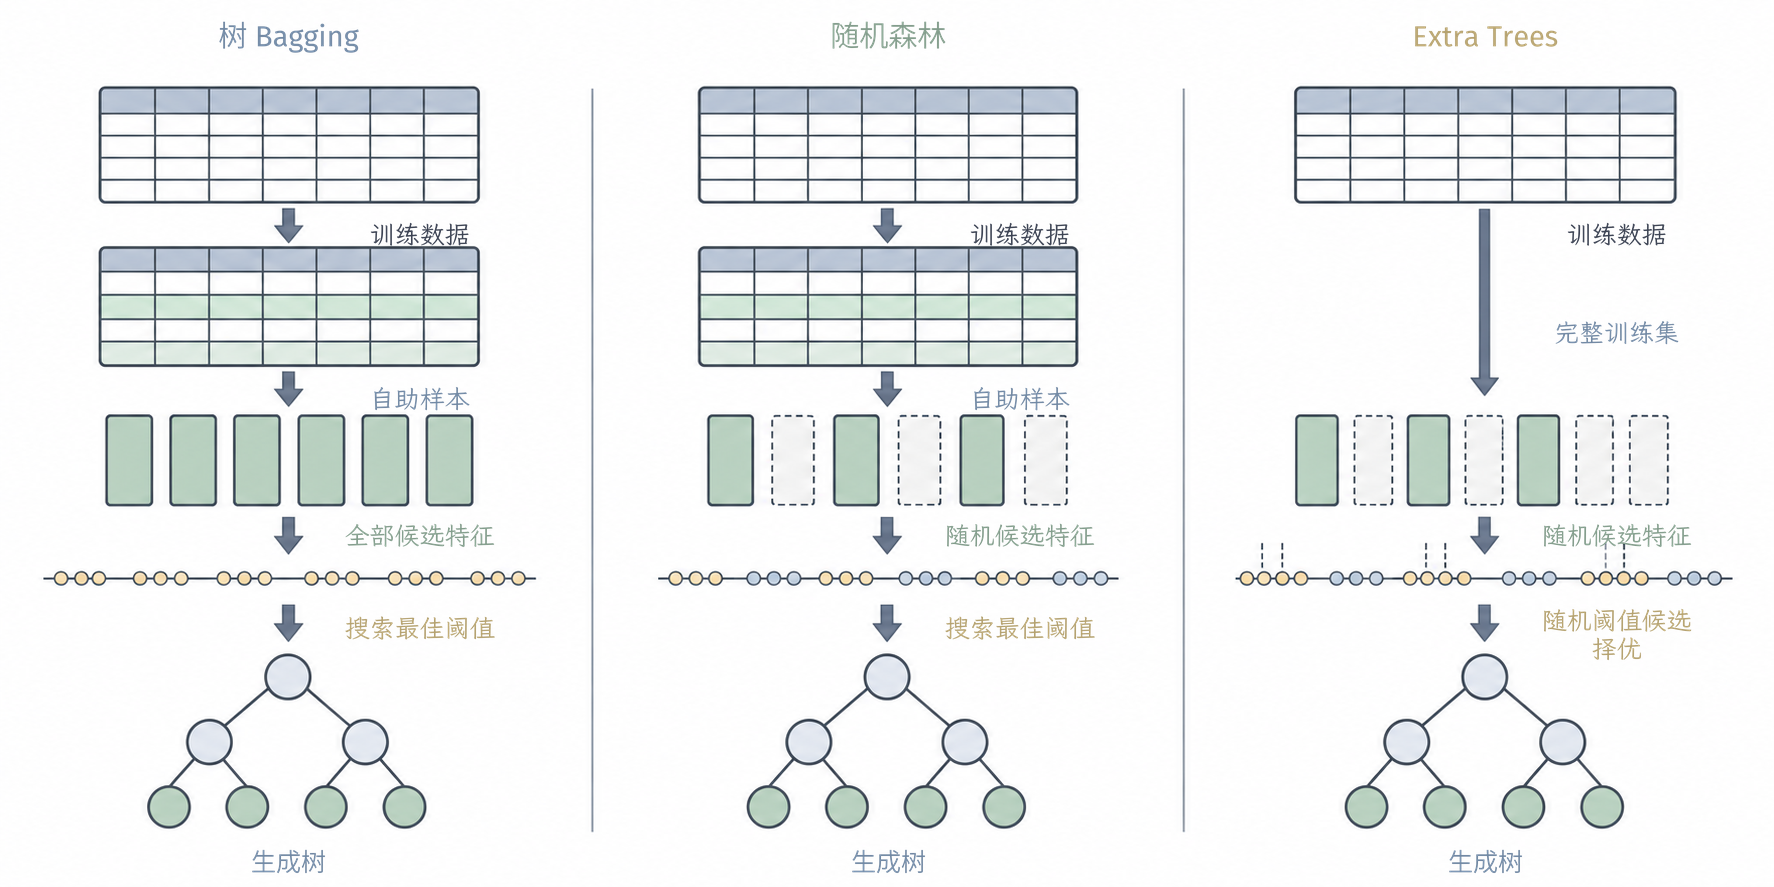
\includegraphics[width=150.199mm]{figures/04-classic-models/00-shared/generated/ensemble-tree-randomization/figure.png}
  \caption{树Bagging、随机森林与Extra Trees的随机化位置。每栏从样本来源出发，依次展示候选特征、候选阈值与成员树；候选选择中的随机性和任务准则约束分别标在相应步骤。每栏首框直接标出训练样本来源：前两栏采用自助采样，Extra Trees栏采用原始方法的完整训练集设定；具体实现也可能额外启用自助采样。}
  \label{fig:ensemble-tree-randomization}
\end{figure*}

三种方法的预测都由树叶输出聚合得到。它们依次改变样本、节点候选特征和候选阈值，训练时仍用任务准则决定分裂与叶值。增加随机化可能减弱共同错误，也可能削弱单树，因此应在相同预算下比较组合预测；表\ref{tab:ensemble-bagging-comparison}列出具体差别。

\begin{table*}[htbp]
  \centering
  \small
  \begin{tabularx}{\linewidth}{@{}>{\raggedright\arraybackslash}p{24mm}*{6}{>{\raggedright\arraybackslash}X}@{}}
    \toprule
    方法 & 样本扰动 & 节点候选特征 & 阈值选择 & 袋外预测 & 成员训练 & 主要边界 \\
    \midrule
    树Bagging & 通常自助采样 & 全部特征 & 在候选中搜索 & 标准自助设定下可用 & 成员间可并行 & 强特征可能使树高度相关 \\
    随机森林 & 通常自助采样 & 随机特征子集 & 在子集内搜索 & 标准自助设定下可用 & 成员间可并行 & 候选数过小会削弱单树 \\
    Extra Trees & 原始方法使用完整训练集；实现可选自助采样 & 随机特征子集 & 生成随机阈值后择优 & 仅在采用自助采样时可用 & 成员间可并行 & 过强随机化会增大单树误差 \\
    \bottomrule
  \end{tabularx}
  \caption{以树为成员时，Bagging、随机森林与Extra Trees的机制比较。表中列出基本构造；比较具体实现时，还需记录抽样设置，并固定树复杂度、成员数和计算预算。}
  \label{tab:ensemble-bagging-comparison}
\end{table*}

原始Extra Trees使用完整训练集，没有标准自助采样形成的袋外预测；若额外启用自助采样，才可按相应未抽中成员构造袋外结果。

Bagging先产生训练差异，再聚合预测以削弱部分波动。固定聚合保留成员共享的遗漏；若希望让新成员针对这些不足训练，就需要根据当前组合产生修正信号。下一节据此转向序贯提升。
